\documentclass[aspectratio=1610,onlymath]{beamer}
% \documentclass[aspectratio=1610,onlymath,handout]{beamer}

\input{macros-lecture}
% Common notation

\usepackage{amsmath,amssymb,amsfonts}
\usepackage{xspace}

\newcommand{\lectureurl}{https://iccl.inf.tu-dresden.de/web/FS2023}

\DeclareMathAlphabet{\mathsc}{OT1}{cmr}{m}{sc} % Let's have \mathsc since the slide style has no working \textsc

% Dual of "phantom": make a text that is visible but intangible
\newcommand{\ghost}[1]{\raisebox{0pt}[0pt][0pt]{\makebox[0pt][l]{#1}}}

\newcommand{\tuple}[1]{\langle{#1}\rangle}
\newcommand{\defeq}{\mathrel{:=}}

%%% Annotation %%%

\usepackage{color}
\newcommand{\todo}[1]{{\tiny\color{red}\textbf{TODO: #1}}}



%%% Old macros below; move when needed

\newcommand{\blank}{\text{\textvisiblespace}} % empty tape cell for TM

% table syntax
\newcommand{\dom}{\textbf{dom}}
\newcommand{\adom}{\textbf{adom}}
\newcommand{\dbconst}[1]{\texttt{"#1"}}
\newcommand{\pred}[1]{\textsf{#1}}
\newcommand{\foquery}[2]{#2[#1]}
\newcommand{\ground}[1]{\textsf{ground}(#1)}
% \newcommand{\foquery}[2]{\{#1\mid #2\}} %% Notation as used in Alice Book
% \newcommand{\foquery}[2]{\tuple{#1\mid #2}}

\newcommand{\quantor}{\mathord{\reflectbox{$\text{\sf{Q}}$}}} % the generic quantor

% logic syntax
\newcommand{\Inter}{\mathcal{I}} %used to denote an interpretation
\newcommand{\Jnter}{\mathcal{J}} %used to denote another interpretation
\newcommand{\Knter}{\mathcal{K}} %used to denote yet another interpretation
\newcommand{\Zuweisung}{\mathcal{Z}} %used to denote a variable assignment

% query languages
\newcommand{\qlang}[1]{{\sf #1}} % Font for query languages
\newcommand{\qmaps}[1]{\textbf{QM}({\sf #1})} % Set of query mappings for a query language

%%% Complexities %%%

\hyphenation{Exp-Time} % prevent "Ex-PTime" (see, e.g. Tobies'01, Glimm'07 ;-)
\hyphenation{NExp-Time} % better that than something else

% \newcommand{\complclass}[1]{{\sc #1}\xspace} % font for complexity classes
\newcommand{\complclass}[1]{\ensuremath{\mathsc{#1}}\xspace} % font for complexity classes

\newcommand{\ACzero}{\complclass{AC$_0$}}
\newcommand{\LogSpace}{\complclass{L}}
\newcommand{\NLogSpace}{\complclass{NL}}
\newcommand{\PTime}{\complclass{P}}
\newcommand{\NP}{\complclass{NP}}
\newcommand{\coNP}{\complclass{coNP}}
\newcommand{\PH}{\complclass{PH}}
\newcommand{\PSpace}{\complclass{PSpace}}
\newcommand{\NPSpace}{\complclass{NPSpace}}
\newcommand{\ExpTime}{\complclass{ExpTime}}
\newcommand{\NExpTime}{\complclass{NExpTime}}
\newcommand{\ExpSpace}{\complclass{ExpSpace}}
\newcommand{\TwoExpTime}{\complclass{2ExpTime}}
\newcommand{\NTwoExpTime}{\complclass{N2ExpTime}}
\newcommand{\ThreeExpTime}{\complclass{3ExpTime}}
\newcommand{\kExpTime}[1]{\complclass{#1ExpTime}}
\newcommand{\kExpSpace}[1]{\complclass{#1ExpSpace}}


\defineTitle{8}{Minimale Automaten}{6. November 2023}

% Notes (2016): did not finish M&N theorem on time, since some extra time was used to
% sketch basic properties of equivalence relations on the board;
% the presentation also lacks an example for the MN DFA construction
% maybe move to next lecture and add more intution on equivalences inline instead

% Notes (2017): still not finished; moved MH to next lecture altogether.
% Things explained on the board:
% - How equivalence relations and equivalence classes look (for slide 10)
% - What compatibility with transitions requires and what the potential problem is (for slide 11)

\begin{document}

\maketitle

\sectionSlideNoHandout{Rückblick}

\begin{frame}[fragile]\frametitle{Darstellungen von Typ-3-Sprachen}

\mbox{}\hspace{-0cm}%
\begin{tikzpicture}[
	decoration=penciline, decorate,
	node distance = 7mm and 9mm,
	mybox/.style args = {#1/#2}{
		draw=#1,% line color
		fill=#2,% fill color
% 		rounded corners,
		thick,
		text width=18mm, minimum height=12mm, inner sep=1mm, 
		align=flush center
	},
	myboxlabel/.style args = {}{
		draw=devilscss,% line color
		fill=strongyellow!40,% fill color
% 		rounded corners,
		thick,
		text width=17mm, minimum height=10mm, inner sep=1.5mm, 
		align=flush center
	},
	myarrow/.style args = {#1}{
		line width=0.8mm,
		draw=#1,%line color
		%-{Triangle[length=2.8mm,width=4mm,fill=#1]},
		->,
		shorten >=0.5mm, shorten <=0.1mm
	}
]
\pgfmathsetseed{7729}
% \draw[help lines] (0,0) grid (5,5);
\node (reg) [decorate,mybox=black/cyan!40] at (2,-0.6) {reguläre Grammatik};
\node (dfa) [decorate,mybox=black/cyan!40] at (0,-4) {DFA};
\node (nfa) [decorate,mybox=black/cyan!40] at (4,-4) {NFA};
\node (re) [decorate,mybox=black/cyan!40] at (6,-0.6) {regulärer Ausdruck};
\node (enfa) [decorate,mybox=black/cyan!40] at (8,-4) {$\epsilon$-NFA};
%
\path[myarrow=devilscss,bend left=20](dfa) edge (reg.180);
% \node (dfareglabel) [decorate,myboxlabel=,text width=19mm] at (-0.4,-0.7) {"`$q_1 \stackrel{\Sterm{a}}{\to} q_2$"' $\leadsto$ "`$q_1\to\Sterm{a}q_2$"'};
%
\path[myarrow=devilscss,-,bend left=20](reg.340) edge[->] (nfa.110);
\path[myarrow=devilscss,-,bend right=20](nfa.130) edge[->] (reg.320);
\node (regnfalabel) [decorate,myboxlabel=] at (1.6,-1.9) {\footnotesize"`$q_1\to\Sterm{a}q_2$"' $\Leftrightarrow$ "`$q_1 \stackrel{\Sterm{a}}{\to} q_2$"'};
%
\draw[myarrow=devilscss](dfa.10)--(nfa.170);
\node (dfanfalabel) [decorate,myboxlabel=,text width=16mm, minimum height=5mm,inner sep=1mm] at (1.95,-3.3) {\scalebox{0.8}{"`DFA${}\subseteq{}$NFA"'}};
%
\draw[myarrow=devilscss](nfa.190)--(dfa.350);
\node (nfadfalabel) [decorate,myboxlabel=,text width=13mm] at (2.1,-5.0) {\footnotesize Potenzm.\-konstr.};
%
\node (sd) [decorate,mybox=black/cyan!40,text width=14mm, minimum height=10mm] at (4,-6.5) {\footnotesize Syntax\-diagramm};
\draw[myarrow=devilscss,<->](sd)--(nfa);
\node (sdnfalabel) [decorate,myboxlabel=, minimum height=0mm,inner sep=1.0mm,text width=19mm] at (5.3,-5.4) {\footnotesize dualer Graph};
%%
\path[myarrow=devilscss,-,bend left=20](nfa.70) edge[->] (re.180);
%
\path[myarrow=devilscss,-,bend left=20](re.0) edge[->] (enfa);
%
\draw[myarrow=devilscss](enfa.190)--(nfa.350);
\draw[myarrow=devilscss](nfa.10)--(enfa.170);
\node (nfaenfalabel) [decorate,myboxlabel=,text width=16mm, minimum height=5mm,inner sep=1mm] at (5.95,-3.3) {\scalebox{0.75}{"`NFA${}\subseteq{}${}$\epsilon$-NFA"'}};
\node (enfanfalabel) [decorate,myboxlabel=,text width=13mm, minimum height=5mm] at (6.1,-4.6) {\footnotesize $\epsilon$-Elim.};
%
\node (nfarelabel) [decorate,myboxlabel=,align=flush left,text width=17mm,inner sep=1mm] at (8.6,-0.7) {\footnotesize 1) komposit.\\2) explizit};

%
{\node (reenfalabel) [decorate,myboxlabel=,align=flush left,text width=18mm,inner sep=1mm] at (5.6,-2.0) {\footnotesize 1) Ersetzung\\2) Dyn. Prog.};}
\end{tikzpicture}

\end{frame}

\sectionSlide{Minimierung von Automaten}

\begin{frame}\frametitle{Automaten verkleinern}

Wir haben bereits Methoden kennengelernt, um Automaten zu vereinfachen:
\begin{itemize}
\item Entfernen von Zuständen, die von keinem Anfangszustand aus erreichbar sind
\item Entfernen von Zuständen, von denen aus kein Endzustand erreicht werden kann
\end{itemize}
\bigskip

\alert{Erhalten wir damit den kleinstmöglichen äquivalenten Automaten?}\bigskip\pause

\redalert{Nein} -- ein einfaches Gegenbeispiel:\bigskip

\examplebox{\emph{Beispiel:} Sei $\Smach{M}$ ein endlicher Automat, bei dem alle Zustände erreichbar sind und
einen Endzustand erreichen können. Der Vereinigungsautomat\footnote{Hierbei müssen die Zustände einer Kopie von $\Smach{M}$ umbenannt werden.} $\Smach{M}\oplus\Smach{M}$ akzeptiert die selbe Sprache, hat nur erreichbare Zustände, aber die doppelte Zustandszahl.
}

\end{frame}


\begin{frame}\frametitle{Ein interessanteres Beispiel}

Der Vereinigungsautomat ist immer ein NFA. Nichtdeterminismus macht es einfach, nichtminimale Automaten zu finden.
\medskip

Interessanter sind nichtminimale DFAs:\medskip

\narrowcentering{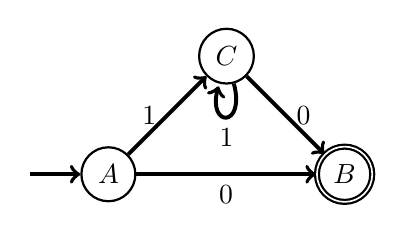
\begin{tikzpicture}[baseline={(current bounding box.center)}]
% \draw[help lines] (0,0) grid (7,2);
\node (s1) [circle,draw=black,thick] at (0,0) {$A$};
\node (s2) [circle,draw=black,thick,double] at (3,0) {$B$};
\node (s3) [circle,draw=black,thick] at (1.5,1.5) {$C$};
%
\path[->,line width=0.5mm](-1,0) edge (s1);
\path[->,line width=0.5mm](s1) edge node[below] {\Sterm{0}} (s2);
\path[->,line width=0.5mm](s1) edge node[left] {\Sterm{1}} (s3);
\path[->,line width=0.5mm](s3) edge node[right] {\Sterm{0}} (s2);
\path[->,line width=0.5mm](s3) edge [loop below] node[below] {\Sterm{1}} (s3);
\end{tikzpicture}}\pause

Dieser DFA hat keine offensichtlich überflüssigen Zustände, aber der folgende kleinere DFA erkennt die selbe Sprache $\Sterm{1}^*\Sterm{0}$:\medskip

\narrowcentering{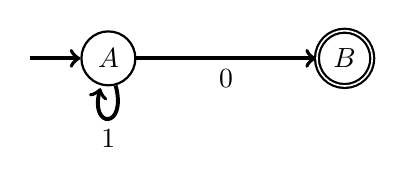
\begin{tikzpicture}[baseline={(current bounding box.center)}]
% \draw[help lines] (0,0) grid (7,2);
\node (s1) [circle,draw=black,thick] at (0,0) {$A$};
\node (s2) [circle,draw=black,thick,double] at (3,0) {$B$};
%
\path[->,line width=0.5mm](-1,0) edge (s1);
\path[->,line width=0.5mm](s1) edge node[below] {\Sterm{0}} (s2);
\path[->,line width=0.5mm](s1) edge [loop below] node[below] {\Sterm{1}} (s1);
\end{tikzpicture}}

\end{frame}

\begin{frame}\frametitle{Automaten minimieren?}

\alert{Wie kann man Automaten weiter minimieren?}
\bigskip

\emph{Beobachtungen:}
\begin{itemize}
\item Zur Erkennung von Wörtern muss der Automat nur seinen aktuellen Zustand kennen
\item Wichtig ist, wohin man vom aktuellen Zustand aus gelangt, wenn man das restliche Wort einliest
\item Es ist nicht relevant, auf welchem Weg man zu diesem Zustand gelangt ist
\end{itemize}\medskip\pause

\emph{Idee:} Zwei Zustände sind gleichwertig, wenn man ausgehend von beiden Zuständen die selbe Sprache akzeptieren kann
\bigskip

$\leadsto$ Gleichwertige Zustände könnten verschmolzen werden \ldots

\end{frame}

\begin{frame}\frametitle{Äquivalenz von Zuständen}

\defbox{Für einen DFA $\Smach{M}=\tuple{Q,\Sigma,\delta,q_0,F}$ und einen Zustand $q\in Q$ sei $\Smach{M}_q=\tuple{Q,\Sigma,\delta,q,F}$ der abgewandelte DFA mit Startzustand $q$.\medskip

Zwei Zustände $p,q\in Q$ sind \redalert{$\Smach{M}$-äquivalent}, in Symbolen \redalert{$p\sim_{\Smach{M}}q$}, wenn gilt:\\
\narrowcentering{$\Slang{L}(\Smach{M}_{p}) = \Slang{L}(\Smach{M}_{q})$}\\[1ex]
das heißt wenn für jedes Wort $w\in\Sigma^*$ gilt:\\[1ex]
\narrowcentering{$\delta(p,w)\in F$ genau dann wenn $\delta(q,w)\in F$.}
}
Wenn der Automat $\Smach{M}$ klar ist, schreiben wir einfach $\sim$ statt $\sim_{\Smach{M}}$.
\medskip\pause

\doodlebox{darkgreen}{%
\emph{Beispiel:}\rule{0pt}{3ex}
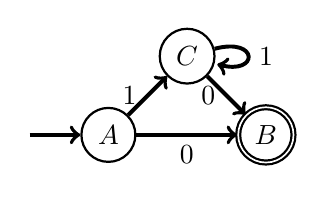
\begin{tikzpicture}[baseline={(s3.center)}]
% \draw[help lines] (0,0) grid (7,2);
\node (s1) [circle,draw=black,thick] at (0,0) {$A$};
\node (s2) [circle,draw=black,thick,double] at (2,0) {$B$};
\node (s3) [circle,draw=black,thick] at (1,1) {$C$};
%
\path[->,line width=0.5mm](-1,0) edge (s1);
\path[->,line width=0.5mm](s1) edge node[below] {\Sterm{0}} (s2);
\path[->,line width=0.5mm](s1) edge node[left] {\Sterm{1}} (s3);
\path[->,line width=0.5mm](s3) edge node[left] {\Sterm{0}} (s2);
\path[->,line width=0.5mm](s3) edge [loop right] node[right] {\Sterm{1}} (s3);
\end{tikzpicture}
\hspace{3mm}
\begin{minipage}[t]{4.7cm}
$\Slang{L}(\Smach{M}_{A}) = \{\Sterm{1}\}^* \{\Sterm{0}\} = \Slang{L}(\Smach{M}_{C})$\\
$\Slang{L}(\Smach{M}_{B}) = \{\epsilon\}$\\[1ex]
$\leadsto$ $A\sim C$\\
\end{minipage}
}

\end{frame}

\begin{frame}\frametitle{Eigenschaften von $\sim_{\Smach{M}}$}

\defbox{ \emph{Definition (kurz):} $q\sim_{\Smach{M}}p$ genau dann wenn $\Slang{L}(\Smach{M}_{p}) = \Slang{L}(\Smach{M}_{q})$.}%
\smallskip\pause

Damit sehen wir leicht:
\begin{itemize}
\item $\sim$ ist \alert{reflexiv}: $q\sim q$
\item $\sim$ ist \alert{symmetrisch}: wenn $q_1\sim q_2$ dann $q_2\sim q_1$
\item $\sim$ ist \alert{transitiv}: wenn $q_1\sim q_2$ und $q_2\sim q_3$ dann $q_1\sim q_3$
\end{itemize}
(jeweils für alle $q,q_1,q_2,q_3\in Q$)
\medskip

\theobox{\emph{Eigenschaft:} $\sim$ ist eine \redalert{Äquivalenzrelation}.}%
\smallskip\pause

Außerdem gilt für alle $\Sterm{a}\in\Sigma$
\begin{itemize}
\item wenn $q_1\sim q_2$ dann $\delta(q_1,\Sterm{a})\sim\delta(q_2,\Sterm{a})$,
falls diese Übergänge definiert sind\\ {\tiny (daher nehmen wir im Folgenden oft eine totale Übergangsfunktion an)

}
\end{itemize}
\smallskip

\theobox{\emph{Eigenschaft:} $\sim$ ist verträglich mit der Übergangsfunktion.}
\smallskip

\end{frame}

\newcommand{\simquot}[1]{#1/_{\!\!{\sim}}}

\begin{frame}\frametitle{Notation für Äquivalenzrelationen}

Wir verwenden die bei Äquivalenzen üblichen Begriffe:
\medskip

\defbox{%
Wir schreiben \redalert{$[q]_{\sim}$} für die \redalert{$\sim$-Äquivalenzklasse} von $q$, d.h.\\[1ex]
%
\narrowcentering{$[q]_{\sim}=\{p\in Q\mid q\sim p\}$.}\\[1ex]
%
Für eine Menge $P\subseteq Q$ schreiben 
wir \redalert{$\simquot{P\!}$} für den \redalert{Quotienten} von $P$ und $\sim$:\\[1ex]
\narrowcentering{$\simquot{P\!} = \{[p]_{\sim}\mid p\in P \}.$}\\
{\tiny (Die Quotientenbildung heißt Faktorisierung; sie entspricht dem "`Verschmelzen"' äquivalenter Zustände.)}
}
Wie immer gilt:
\begin{itemize}
\item Wenn $q_1\sim q_2$ dann $[q_1]_{\sim}=[q_2]_{\sim}$
\item Unterschiedliche Äquivalenzklassen sind disjunkt, d.h. $[q_1]_{\sim}\neq [q_2]_{\sim}$ impliziert $[q_1]_{\sim}\cap [q_2]_{\sim}=\emptyset$
\item Die Äquivalenzklassen partitionieren $Q$, d.h. $Q$ ist die Vereinigung der (disjunkten) Klassen
\end{itemize}
% Offensichtlich gibt es nur endlich viele Äquivalenzklassen, da $Q$ endlich ist

\end{frame}

\begin{frame}\frametitle{Der Quotientenautomat}

Wir vereinfachen Automaten, indem wir äquivalente Zustände verschmelzen:

\defbox{Für einen DFA $\Smach{M}=\tuple{Q,\Sigma,\delta,q_0,F}$ mit totaler Übergangsfunktion ist der 
\redalert{Quotientenautomat $\simquot{\Smach{M}}$} gegeben durch
$\simquot{\Smach{M}}=\tuple{\simquot{Q},\Sigma,\delta_{\sim},[q_0]_{\sim_{\Smach{M}}},\simquot{F\!}}$ wobei gilt:%
\begin{itemize}
\item $\simquot{Q} = \{[q]_{\sim}\mid q\in Q\}$
\item $\delta_{\sim}([q]_{\sim},\Sterm{a}) = [\delta(q,\Sterm{a})]_{\sim}$
\item $\simquot{F\!} = \{[q]_{\sim}\mid q\in F\}$
\end{itemize}
}\pause

Diese Definition ergibt Sinn, da gilt:
\begin{itemize}
\item wenn $[q]_{\sim}=[p]_{\sim}$ dann $[\delta(q,\Sterm{a})]_{\sim_{\Smach{M}}}=[\delta(p,\Sterm{a})]_{\sim_{\Smach{M}}}$ (Verträglichkeit von $\sim$ und $\delta$; benötigt totale Übergangsfunktion)
\item wenn $[q]_{\sim}=[p]_{\sim}$ dann ~~$q\in F$ gdw. $p\in F$ ~~(Übung)
\end{itemize}
$\leadsto$ Definition unabhängig vom gewählten Repräsentanten von $[q]_{\sim}$

\end{frame}


\begin{frame}\frametitle{Beispiel}

\narrowcentering{\begin{tikzpicture}[baseline={(current bounding box.center)}]
\draw[dashed,fill=strongyellow!30] (-0.8,-0.9) rectangle node[above,yshift=-1.50cm,xshift=-0.0cm] {\footnotesize$[A]_\sim = [C]_\sim =\{A,C\}$}(2.0,2.0);
\draw[dashed,fill=strongyellow!30] (2.2,-0.9) rectangle node[above,yshift=-1cm,xshift=-0.0cm] {\footnotesize$[B]_\sim =\{B\}$}(3.6,1.0);
% \draw[help lines] (0,0) grid (7,2);
\node (s1) [circle,draw=black,thick] at (0,0) {$A$};
\node (s2) [circle,draw=black,thick,double] at (3,0) {$B$};
\node (s3) [circle,draw=black,thick] at (1.5,1.5) {$C$};
%
\path[->,line width=0.5mm](-1,0) edge (s1);
\path[->,line width=0.5mm](s1) edge node[below] {\Sterm{0}} (s2);
\path[->,line width=0.5mm](s1) edge node[left] {\Sterm{1}} (s3);
\path[->,line width=0.5mm](s3) edge node[right] {\Sterm{0}} (s2);
\path[->,line width=0.5mm](s3) edge [loop above] node[above] {\Sterm{1}} (s3);
\end{tikzpicture}}\pause\bigskip

\narrowcentering{Es ergibt sich der folgende Quotientenautomat:}\medskip

\narrowcentering{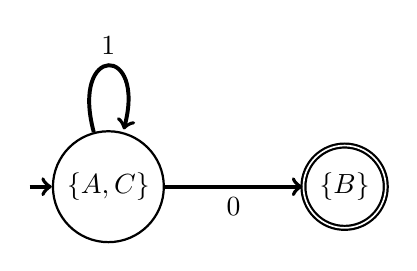
\begin{tikzpicture}[baseline={(current bounding box.center)}]
% \draw[help lines] (0,0) grid (7,2);
\node (s1) [circle,draw=black,thick] at (0,0) {$\{A,C\}$};
\node (s2) [circle,draw=black,thick,double] at (3,0) {$\{B\}$};
%
\path[->,line width=0.5mm](-1,0) edge (s1);
\path[->,line width=0.5mm](s1) edge node[below] {\Sterm{0}} (s2);
\path[->,line width=0.5mm](s1) edge [loop above] node[above] {\Sterm{1}} (s1);
\end{tikzpicture}}

\end{frame}


\begin{frame}\frametitle{Korrektheit Quotientenautomat}

\theobox{\emph{Satz:} Für jeden totalen DFA $\Smach{M}$ gilt $\Slang{L}(\Smach{M})=\Slang{L}(\simquot{\Smach{M}})$.}

\emph{Beweis:}
Für alle $w\in\Sigma^*$ gilt:
\[\begin{array}{l@{~~\text{ gdw. }~~}ll}
 w\in \Slang{L}(\Smach{M})
	& \delta(q_0,w)\in F & \textcolor{devilscss}{\text{laut Definition}}\\\pause
	& [\delta(q_0,w)]_\sim\in \simquot{F} & \textcolor{devilscss}{\text{wie zuvor bemerkt (Übung)}} \\\pause
	& \delta_\sim([q_0]_\sim,w)\in \simquot{F} & \textcolor{devilscss}{\text{Lemma $\varheartsuit$}}\\\pause
	& w\in \Slang{L}(\simquot{\Smach{M}}) & \textcolor{devilscss}{\text{laut Definition}}
\end{array}
\]\pause

\codebox{Lemma $\varheartsuit$: Für beliebige $q\in Q$ und $w\in\Sigma^*$ gilt:\\[1ex]
\narrowcentering{$[\delta(q,w)]_\sim = \delta_\sim([q]_\sim,w)$.}}

Beweis durch Induktion über $|w|$ (Übung)\qed

\end{frame}


\begin{frame}\frametitle{Berechnung von $\sim_{\Smach{M}}$}

\alert{Wie kann man $\sim_{\Smach{M}}$ praktisch ermitteln?}
\bigskip 

Zuvor bemerkten wir:
\theobox{\vspace{-1ex}
\begin{enumerate}[(1)]
\item Wenn $q_1\sim q_2$ dann $q_1\in F$ gdw. $q_2 \in F$
\item Wenn $q_1\sim q_2$ dann $\delta(q_1,\Sterm{a})\sim\delta(q_2,\Sterm{a})$
\end{enumerate}}%
\bigskip 

Umgekehrt gilt also:
\theobox{\vspace{-1ex}
\begin{enumerate}[(1')]
\item Wenn $q_1\in F$ und $q_2 \notin F$ dann $q_1\not\sim q_2$
\item Wenn $\delta(q_1,\Sterm{a})\not\sim\delta(q_2,\Sterm{a})$ dann $q_1\not\sim q_2$
\end{enumerate}}%
\bigskip 

Tatsächlich ist $\not\sim$ die \alert{kleinste Relation}, die (1') und (2') erfüllt.
\medskip

$\leadsto$ Wir können $\not\sim$ (und damit auch $\sim$) durch rekursive Anwendung der Regeln (1') und (2') berechnen


\end{frame}


\begin{frame}\frametitle{Algorithmus zur Berechnung von $\sim_{\Smach{M}}$}

\codebox{%
\emph{Eingabe:} DFA $\Smach{M}=\tuple{Q,\Sigma,\delta,q_0,F}$\\
\emph{Ausgabe:} $\sim_{\Smach{M}}$\\%[1ex]
%
\begin{itemize}
\item Initialisiere ${\not\sim}\defeq\emptyset$
\item (Regel 1) Für jedes Paar von Zuständen $\tuple{q,p}\in Q\times Q$:\\
	falls $q\in F$ und $p\notin F$, dann "`speichere $q\not\sim p$"'
	% ${\not\sim}\defeq{\not\sim}\cup\{\tuple{q,p},\tuple{p,q}\}$
\item (Regel 2) Für jedes Paar $\tuple{q,p}\in Q\times Q\setminus {\not\sim}$ und jedes $\Sterm{a}\in\Sigma$:\\
	falls $\delta(q,\Sterm{a})\not\sim\delta(p,\Sterm{a})$ dann "`speichere $q\not\sim p$"'
% 	${\not\sim}\defeq{\not\sim}\cup\{\tuple{q,p},\tuple{p,q}\}$
\item Wiederhole die Anwendung von Regel 2 solange, bis es keine Änderungen mehr gibt
\item Das Ergebnis ist $(Q\times Q)\setminus {\not\sim}$
\end{itemize}
}

\end{frame}


\begin{frame}\frametitle{Darstellung von $\not\sim$ im Algorithmus}

Die Anweisung "`speichere $q\not\sim p$"' könnte umgesetzt werden als:\\[1ex]
\narrowcentering{${\not\sim}\defeq{\not\sim}\cup\{\tuple{q,p},\tuple{p,q}\}$}
\bigskip

Es ist aber nicht nötig, alle Paare in ${\not\sim}$ einzeln zu speichern:
\begin{itemize}
\item $\not\sim$ ist irreflexiv, d.h. man muss $q\not\sim q$ nicht betrachten
\item $\not\sim$ ist symmetrisch, d.h. man muss jeweils nur entweder $q\not\sim p$ oder $p\not\sim q$ betrachten\pause
\end{itemize}
$\leadsto$ Halb-Tabelle genügt zum Eintragen der möglichen Paare\medskip

\examplebox{
\begin{minipage}{6cm}\begin{flushleft}
Beispiel: Für einen DFA mit Zuständen $Q=\{A,B,C,D,E\}$ genügt eine Tabelle mit zehn Feldern (statt $5^2=25$).\\[1ex]

{\tiny (dazu reihen wir Zustände vertikal in umgekehrter Reihenfolge)}
\end{flushleft}
\end{minipage}
\narrowcentering{\scalebox{0.8}{%
\begin{tabular}{c|c|c|c|c|}
 \multicolumn{1}{c}{}  & \multicolumn{1}{c}{A} & \multicolumn{1}{c}{B} & \multicolumn{1}{c}{C} & \multicolumn{1}{c}{D}  \\\cline{2-5}
 E &   &   &   &    \\\cline{2-5}
 D &   &   &        \\\cline{2-4} 
 C &   &            \\\cline{2-3}
 B &                \\\cline{2-2}
\end{tabular}}}
}

\end{frame}

\newcommand{\hicell}[1]{\only<#1|handout:0>{\cellcolor{strongyellow}}}
\newcommand{\upcell}[2]{\only<#1|handout:0>{\cellcolor{strongyellow}}\only<#1->{#2}}
\newcommand{\locell}[1]{\only<#1|handout:0>{\cellcolor{darkgreen!20}}}

\begin{frame}[t]\frametitle{Beispiel Quotientenautomat}

\begin{minipage}{7cm}
\narrowcentering{\begin{tikzpicture}[baseline={(current bounding box.center)}]
% \draw[help lines] (0,0) grid (7,2);
\node (s0) [circle,draw=black,thick,onslide={<2,6,7,13-15,18,19>{fill=strongyellow}}] at (0,0) {$A$};
\node (s1) [circle,draw=black,thick,onslide={<3,8-10,16-19>{fill=strongyellow}}] at (2,0) {$B$};
\node (s2) [circle,draw=black,thick,onslide={<4,11-17>{fill=strongyellow}}] at (1.0,1.5) {$C$};
\node (s3) [circle,draw=black,thick,onslide={<5-12>{fill=strongyellow}}] at (3,1.5) {$D$};
\node (s4) [circle,draw=black,thick,double,onslide={<2-5>{fill=strongyellow}}] at (4,0) {$E$};
%
\path[->,line width=0.5mm](-1,0) edge (s0);
\path[->,line width=0.5mm,onslide={<7,14,19>{dashed,darkred}}](s0) edge node[below] {\Sterm{0}} (s1);
\path[->,line width=0.5mm,onslide={<9,17,19>{dashed,darkred}}](s1) edge node[below] {\Sterm{0}} (s4);
\path[->,line width=0.5mm,bend right,onslide={<10>{dashed,darkred}}](s1) edge node[right] {\Sterm{1}} (s2);
\path[->,line width=0.5mm,onslide={<15>{dashed,darkred}}](s0) edge node[left] {\Sterm{1}} (s2);
\path[->,line width=0.5mm,onslide={<15>{dashed,darkred}}](s2) edge[loop below,in=270,out=310,min distance=5mm] node[below] {\Sterm{1}} (s2);
\path[->,line width=0.5mm,onslide={<12,14,17>{dashed,darkred}}](s2) edge node[above] {\Sterm{0}} (s3);
\path[-,line width=0.5mm,onslide={<10>{dashed,darkred}}](s3) edge[bend right=75] (0,1.5)
	 (0,1.5) edge[->] node[left] {\Sterm{1}} (s0);
\path[->,line width=0.5mm,onslide={<7,9,12>{dashed,darkred}}](s3) edge node[above] {\Sterm{0}} (s4);
\path[->,line width=0.5mm](s4) edge [loop right] node[right] {\Sterm{0},\Sterm{1}} (s4);
\end{tikzpicture}}
\end{minipage}%
\begin{minipage}{4.9cm}
\begin{enumerate}[(1)]
\item $q\in F$ und $p\notin F$ \\impliziert $q\not\sim p$
\item $\delta(q,\Sterm{a})\not\sim\delta(p,\Sterm{a})$ \\impliziert $q\not\sim p$
\end{enumerate}
\end{minipage}
\medskip

Wir tragen in der Tabelle jeweils die Wörter ein, die $q\not\sim p$ zeigen:\medskip

\begin{tabular}{c|c|c|c|c|}
 \multicolumn{1}{c}{}  & \multicolumn{1}{c}{A} & \multicolumn{1}{c}{B} & \multicolumn{1}{c}{C} & \multicolumn{1}{c}{D}  \\\cline{2-5}
 E & \upcell{2}{$\epsilon$}  & \upcell{3}{$\epsilon$}\locell{7}  & \upcell{4}{$\epsilon$}  &  \upcell{5}{$\epsilon$}\locell{12}\locell{17} \\\cline{2-5}
 D & \hicell{6}\upcell{7}{$\Sterm{0}$} & \hicell{8-10}\locell{14}  &  \hicell{11}\upcell{12}{$\Sterm{0}$} \\\cline{2-4} 
 C & \locell{10}\hicell{13-15} & \hicell{16}\upcell{17}{$\Sterm{0}$}  \\\cline{2-3}
 B & \hicell{18}\upcell{19}{$\Sterm{0}$}  \\\cline{2-2}
\end{tabular}~~~
\begin{minipage}{6cm}
\only<20->{Weitere Abarbeitung von Regel (2) führt nicht mehr zu Änderungen
\begin{align*}
{\sim} ={}&\{ \tuple{B,D},\tuple{D,B},\tuple{A,C},\tuple{C,A}\}\cup{}\\
	& \{\tuple{q,q}\mid q\in Q\}
\end{align*}}
\end{minipage}

\end{frame}

\begin{frame}[t]\frametitle{Beispiel Quotientenautomat}

\begin{minipage}{7cm}
\narrowcentering{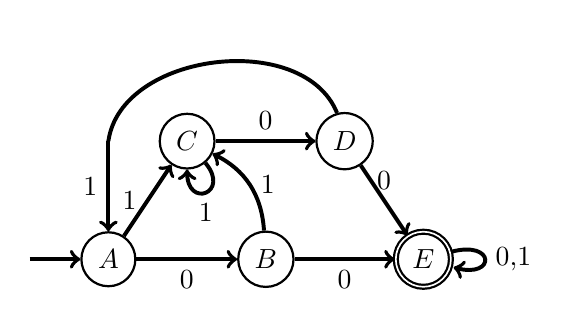
\begin{tikzpicture}[baseline={(current bounding box.center)}]
% \draw[help lines] (0,0) grid (7,2);
\node (s0) [circle,draw=black,thick] at (0,0) {$A$};
\node (s1) [circle,draw=black,thick] at (2,0) {$B$};
\node (s2) [circle,draw=black,thick] at (1.0,1.5) {$C$};
\node (s3) [circle,draw=black,thick] at (3,1.5) {$D$};
\node (s4) [circle,draw=black,thick,double] at (4,0) {$E$};
%
\path[->,line width=0.5mm](-1,0) edge (s0);
\path[->,line width=0.5mm](s0) edge node[below] {\Sterm{0}} (s1);
\path[->,line width=0.5mm](s1) edge node[below] {\Sterm{0}} (s4);
\path[->,line width=0.5mm,bend right](s1) edge node[right] {\Sterm{1}} (s2);
\path[->,line width=0.5mm](s0) edge node[left] {\Sterm{1}} (s2);
\path[->,line width=0.5mm](s2) edge[loop below,in=270,out=310,min distance=5mm] node[below] {\Sterm{1}} (s2);
\path[->,line width=0.5mm](s2) edge node[above] {\Sterm{0}} (s3);
\path[-,line width=0.5mm](s3) edge[bend right=75] (0,1.5)
	 (0,1.5) edge[->] node[left] {\Sterm{1}} (s0);
\path[->,line width=0.5mm](s3) edge node[above] {\Sterm{0}} (s4);
\path[->,line width=0.5mm](s4) edge [loop right] node[right] {\Sterm{0},\Sterm{1}} (s4);
\end{tikzpicture}}
\end{minipage}%
\bigskip

Quotientenautomat:\medskip

\narrowcentering{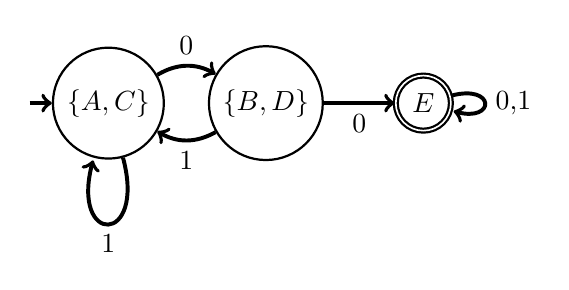
\begin{tikzpicture}[baseline={(current bounding box.center)}]
% \draw[help lines] (0,0) grid (7,2);
\node (s0) [circle,draw=black,thick] at (0,0) {$\{A,C\}$};
\node (s1) [circle,draw=black,thick] at (2,0) {$\{B,D\}$};
% \node (s2) [circle,draw=black,thick] at (1.0,1.5) {$C$};
% \node (s3) [circle,draw=black,thick] at (3,1.5) {$D$};
\node (s4) [circle,draw=black,thick,double] at (4,0) {$E$};
%
\path[->,line width=0.5mm](-1,0) edge (s0);
\path[->,line width=0.5mm,bend left](s0) edge node[above] {\Sterm{0}} (s1);
\path[->,line width=0.5mm](s1) edge node[below] {\Sterm{0}} (s4);
% \path[->,line width=0.5mm,bend right](s1) edge node[right] {\Sterm{1}} (s2);
\path[->,line width=0.5mm,bend left](s1) edge node[below] {\Sterm{1}} (s0);
\path[->,line width=0.5mm](s0) edge[loop below] node[below] {\Sterm{1}} (s0);
\path[->,line width=0.5mm](s4) edge [loop right] node[right] {\Sterm{0},\Sterm{1}} (s4);
\end{tikzpicture}}

\end{frame}


\begin{frame}\frametitle{Reduktion von Automaten}

Wir können das bisher gezeigte zusammenfassen:

\defbox{Sei $\Smach{M}$ ein DFA mit totaler Übergangsfunktion.
Der \redalert{reduzierte Automat $\Smach{M}_r$} ergibt sich durch folgende Schritte:
\begin{enumerate}[(1)]
\item Entferne alle unerreichbaren Zustände aus $\Smach{M}$
\item Berechne den Quotientenautomaten
\end{enumerate}
}\pause

Dieses Verfahren erzeugt den gewünschten minimalen DFA:

\theobox{\emph{Satz:} $\Smach{M}_r$ ist bezüglich der Zustandsmenge der minimale DFA mit totaler Übergangsfunktion, der die Sprache $\Slang{L}(\Smach{M})$ erkennt.}\pause

Zudem stellt sich heraus, dass dieser minimale DFA eindeutig ist:

\theobox{\emph{Satz:} Alle minimalen DFA mit totaler Übergangsfunktion, die $\Slang{L}(\Smach{M})$ erkennen, sind bis auf Umbenennung von Zuständen gleich (sie sind \alert{isomorph}). Daher hängt $\Smach{M}_r$ nur von $\Slang{L}(\Smach{M})$ ab, nicht von $\Smach{M}$.}

\end{frame}

\begin{frame}\frametitle{Korrektheit Minimalautomat}

\theobox{\emph{Satz:} $\Smach{M}_r$ ist bezüglich der Zustandsmenge der minimale DFA mit totaler Übergangsfunktion, der die Sprache $\Slang{L}(\Smach{M})$ erkennt.}

\emph{Beweisplan:}
\begin{enumerate}%[({Behauptung} 1)]
\item $\Smach{M}_r$ erkennt $\Slang{L}(\Smach{M})$: Dies folgt aus der Korrektheit der Quotientenbildung bei Automaten
\item $\Smach{M}_r$ ist minimal für diese Eigenschaft: Wir werden dies in mehreren Schritten zeigen:
\begin{itemize}
\item Wir konstruieren einen weiteren minimalen Automaten $\Smach{M}_{\Slang{L}}$ direkt aus $\Slang{L}$
\item Wir zeigen, dass $\Smach{M}_{\Slang{L}}$ und $\Smach{M}_r$ bis auf Umbenennung von Zuständen gleich sind
\end{itemize}
Damit ist auch die behauptete Eindeutigkeit gezeigt.
\end{enumerate}

\end{frame}

\begin{frame}\frametitle{Die Nerode-Rechtskongruenz}

\defbox{Für eine Sprache $\Slang{L}\subseteq\Sigma^*$ ist die
\redalert{Nerode-Rechtskongruenz} $\simeq_{\Slang{L}}$
wie folgt definiert. Für Wörter $u,v\in\Sigma^*$ sei $u\simeq_{\Slang{L}}v$ wenn
gilt:\\[1ex]
\narrowcentering{für alle $w\in\Sigma^*$ gilt $uw\in\Slang{L}$ genau dann wenn $vw\in\Slang{L}$.}
}
Wenn $\Slang{L}$ klar ist, dann schreiben wir einfach $\simeq$ statt $\simeq_{\Slang{L}}$

\pause\medskip

\alert{Anders gesagt:} zwei Wörter $v$ und $u$ sind kongruent, wenn man in einem Wort das Präfix $v$ gegen $u$ vertauschen kann, ohne dass dies den Status des Worts bezüglich $\Slang{L}$ verändert
\bigskip

Dies kann mit der Idee der Zustandsäquivalenz verglichen werden:

\theobox{(Rückblick) Für Zustände $p,q\in Q$ sei $p\sim q$ wenn gilt:\\[1ex]
\narrowcentering{für alle $w\in\Sigma^*$ gilt $\delta(p,w)\in F$ genau dann wenn $\delta(q,w)\in F$.}
}

\end{frame}

\begin{frame}\frametitle{Eigenschaften von $\simeq$}

\defbox{\emph{Definition (kurz):} $u\simeq_{\Slang{L}}v$ wenn
für alle $w\in\Sigma^*$ gilt: $uw\in\Slang{L}$ genau dann wenn $vw\in\Slang{L}$.
}%
\smallskip\pause

Damit sehen wir leicht:
\begin{itemize}
\item $\simeq$ ist \alert{reflexiv}: $u\simeq u$
\item $\simeq$ ist \alert{symmetrisch}: wenn $u\simeq v$ dann $v\simeq u$
\item $\simeq$ ist \alert{transitiv}: wenn $u\simeq v$ und $v\simeq w$ dann $u\simeq w$
\end{itemize}
(jeweils für alle $u,v,w\in \Sigma^*$)
\medskip

\theobox{Eigenschaft: $\simeq$ ist eine \redalert{Äquivalenzrelation}.}%
\smallskip\pause

Außerdem gilt für alle $w\in\Sigma^*$
\begin{itemize}
\item wenn $u\simeq v$ dann $uw\simeq vw$
\end{itemize}
\smallskip

\theobox{Eigenschaft: $\simeq$ ist verträglich mit der Konkatenation von rechts.}%
\smallskip

Dies rechtfertigt die Bezeichnung \alert{Rechtskongruenz}.

\end{frame}


\begin{frame}[t]\frametitle{Beispiel}

\examplebox{Die Sprache $\Slang{L}=\{\Sterm{a}\}^*\{\Sterm{b}\}^*$ hat die folgenden\\ Nerode-Äquivalenzklassen:

\only<2->{
\begin{itemize}
\item $[\epsilon]_{\simeq} = \{\Sterm{a}\}^*$: für jedes $v\in[\epsilon]_{\simeq}$ ist $vw\in\Slang{L}$ gdw. $w\in\Slang{L}$
\only<3->{\item $[\Sterm{b}]_{\simeq} = \{\Sterm{a}\}^*\{\Sterm{b}\}^+$: für jedes $v\in[\Sterm{b}]_{\simeq}$ ist $vw\in\Slang{L}$ gdw. $w\in\{\Sterm{b}\}^*$}
\only<4->{\item $[\Sterm{ba}]_{\simeq} = \Sigma^*\setminus\Slang{L}$: für jedes $v\in[\Sterm{ba}]_{\simeq}$ ist $vw\notin\Slang{L}$ für alle $w\in\Sigma^*$}
\end{itemize}}
}

\only<5->{
\examplebox{Die endliche Sprache $\Slang{L}=\{\Sterm{a},\Sterm{ab},\Sterm{ba}\}$ hat die folgenden\\ Nerode-Äquivalenzklassen:

\only<6->{
\begin{itemize}
\item $[\epsilon]_{\simeq} = \{\epsilon\}$: $\epsilon w\in\Slang{L}$ gdw. $w\in\Slang{L}$
\only<7->{\item $[\Sterm{a}]_{\simeq} = \{\Sterm{a}\}$: $\Sterm{a}w\in\Slang{L}$ gdw. $w\in\{\epsilon,\Sterm{b}\}$}
\only<8->{\item $[\Sterm{b}]_{\simeq} = \{\Sterm{b}\}$: $\Sterm{b}w\in\Slang{L}$ gdw. $w = \Sterm{a}$}
\only<9->{\item $[\Sterm{ab}]_{\simeq} = \{\Sterm{ab},\Sterm{ba}\}$: für jedes $v\in[\Sterm{ab}]_{\simeq}$ ist $vw\in\Slang{L}$ gdw. $w=\epsilon$}
\only<10->{\item $[\Sterm{bb}]_{\simeq} = \Sigma^*\setminus\{\epsilon,\Sterm{a},\Sterm{b},\Sterm{ab},\Sterm{ba}\}$: für jedes $v\in[\Sterm{bb}]_{\simeq}$ ist $vw\notin\Slang{L}$ für alle $w\in\Sigma^*$}
\end{itemize}}
}}

\end{frame}

\begin{frame}[t]\frametitle{Beispiel (2)}

\examplebox{Die Sprache $\Slang{L}=\{\Sterm{a}^n \Sterm{b}^n\mid n\geq 0\}$ hat die folgenden\\ Nerode-Äquivalenzklassen:

\only<2->{
\begin{itemize}
\item $[\epsilon]_{\simeq} = \{\epsilon\}$: $\epsilon w\in\Slang{L}$ gdw. $w\in\Slang{L}$
\only<3->{\item $[\Sterm{a}]_{\simeq} = \{\Sterm{a}\}$: $\Sterm{a}w\in\Slang{L}$ gdw. $w\in\{\Sterm{a}^n \Sterm{b}^{n+1}\mid n\geq 0\}$}
\only<4->{\item $[\Sterm{aa}]_{\simeq} = \{\Sterm{aa}\}$: $\Sterm{aa}w\in\Slang{L}$ gdw. $w\in\{\Sterm{a}^n \Sterm{b}^{n+2}\mid n\geq 0\}$}
\only<5->{\item $[\Sterm{aaa}]_{\simeq} = \{\Sterm{aaa}\}$: $\Sterm{aaa}w\in\Slang{L}$ gdw. $w\in\{\Sterm{a}^n \Sterm{b}^{n+3}\mid n\geq 0\}$}
\only<6->{\item \ldots unendlich viele Äquivalenzklassen $[\Sterm{a}^n]_{\simeq}=\{\Sterm{a}^n\}$}
\end{itemize}
}
	\only<7->{Es gibt weitere Formen von Äquivalenzklassen, z.B. $[\Sterm{aab}]=\{\Sterm{a}^{n+1} \Sterm{b}^{n}\mid n\geq 0\}$.}
}\bigskip

\only<8->{$\leadsto$ $\Slang{L}=\{\Sterm{a}^n \Sterm{b}^n\mid n\geq 0\}$ hat unendlich viele Nerode-Äquivalenzklassen}

\end{frame}

\begin{frame}[t]\frametitle{$\simeq$ und reguläre Sprachen}

Wir werden zeigen, dass jede reguläre Sprache endlich viele $\simeq$-Äquivalenzklassen hat.
\medskip\pause

Es gilt sogar noch etwas stärkeres:\medskip

\theobox{\emph{Satz (Myhill \& Nerode):} Eine Sprache $\Slang{L}$ ist genau dann regulär, wenn $\simeq_{\Slang{L}}$ endlich viele Äquivalenzklassen hat.}

\emph{Beweis:} Siehe nächste Vorlesung.
\bigskip


\end{frame}


\begin{frame}\frametitle{Zusammenfassung und Ausblick}

Im \redalert{Quotientenautomaten} werden äquivalente Zustände verschmolzen
\bigskip

\redalert{Äquivalente Zustände} in einem (totalen) DFA können rekursiv ermittelt werden
\bigskip

Der \redalert{Satz von Myhill und Nerode} charakterisiert reguläre Sprachen
% und liefert einen direkt konstruierten DFA für einen Sprache
\bigskip

\anybox{yellow}{
Offene Fragen:
\begin{itemize}
\item Wie geht es weiter mit dem Beweis der Eindeutigkeit des Minimalautomaten?
\item Wie aufwändig sind die verschiedenen Konstruktionen auf regulären Sprachen?
\item Welche Sprachen sind nicht regulär?
\end{itemize}
}

\end{frame}


\end{document}
